%%%
% Plantilla de Presentación
% Modificación de una plantilla de Latex de LaTeXTemplates para adaptarla 
% al castellano y a las necesidades de escribir informática y matemáticas.
%
% Editada por: Mario Román
%
% License:
% CC BY-NC-SA 3.0 (http://creativecommons.org/licenses/by-nc-sa/3.0/)
%%%

%%%%%%%%%%%%%%%%%%%%%%%%%%%%%%%%%%%%%%%%%
% Beamer Presentation
% LaTeX Template
% Version 1.0 (10/11/12)
%
% This template has been downloaded from:
% http://www.LaTeXTemplates.com
%
% License:
% CC BY-NC-SA 3.0 (http://creativecommons.org/licenses/by-nc-sa/3.0/)
%
%%%%%%%%%%%%%%%%%%%%%%%%%%%%%%%%%%%%%%%%%

%----------------------------------------------------------------------------------------
%	PAQUETES Y CONFIGURACIÓN DEL DOCUMENTO
%----------------------------------------------------------------------------------------

\documentclass{beamer}
\geometry{paperwidth=140mm,paperheight=105mm}

%% Configuración de la presentación
\mode<presentation> {
  %%% Selección de estilo
  % The Beamer class comes with a number of default slide themes
  % which change the colors and layouts of slides. Below this is a list
  % of all the themes, uncomment each in turn to see what they look like.

  %\usetheme{default}
  %\usetheme{AnnArbor}
  %\usetheme{Antibes}
  %\usetheme{Bergen}
  %\usetheme{Berkeley}
  %\usetheme{Berlin}
  %\usetheme{Boadilla}
  %\usetheme{CambridgeUS}
  %\usetheme{Copenhagen}
  %\usetheme{Darmstadt}
  \usetheme{Dresden}
  %\usetheme{Frankfurt}
  %\usetheme{Goettingen}
  %\usetheme{Hannover}
  %\usetheme{Ilmenau}
  %\usetheme{JuanLesPins}
  %\usetheme{Luebeck}
  %\usetheme{Madrid}
  %\usetheme{Malmoe}
  %\usetheme{Marburg}
  %\usetheme{Montpellier}
  %\usetheme{PaloAlto}
  %\usetheme{Pittsburgh}
  %\usetheme{Rochester}
  %\usetheme{Singapore}
  %\usetheme{Szeged}
  %\usetheme{Warsaw}

  %% Selección de color
  % As well as themes, the Beamer class has a number of color themes
  % for any slide theme. Uncomment each of these in turn to see how it
  % changes the colors of your current slide theme.

  %\usecolortheme{albatross}
  \usecolortheme{beaver}
  %\usecolortheme{beetle}
  %\usecolortheme{crane}
  %\usecolortheme{dolphin}
  %\usecolortheme{dove}
  %\usecolortheme{fly}
  %\usecolortheme{lily}
  %\usecolortheme{orchid}
  %\usecolortheme{rose}
  %\usecolortheme{seagull}
  %\usecolortheme{seahorse}
  %\usecolortheme{whale}
  %\usecolortheme{wolverine}

  %% Configuración del pie de línea
  %\setbeamertemplate{footline} % To remove the footer line in all slides uncomment this line
  %\setbeamertemplate{footline}[page number] % To replace the footer line in all slides with a simple slide count uncomment this line
  %\setbeamertemplate{navigation symbols}{} % To remove the navigation symbols from the bottom of all slides uncomment this line
}

%% Fuentes de tamaño arbitrario
\usepackage{lmodern}

%% Gráficos
\usepackage{graphicx} % Allows including images
\usepackage{booktabs} % Allows the use of \toprule, \midrule and \bottomrule in tables

%%% Castellano.
% noquoting: Permite uso de comillas no españolas.
% lcroman: Permite la enumeración con numerales romanos en minúscula.
% fontenc: Usa la fuente completa para que pueda copiarse correctamente del pdf.
\usepackage[spanish,es-noquoting,es-lcroman]{babel}
\usepackage[utf8]{inputenc}
\usepackage[T1]{fontenc}
\selectlanguage{spanish}

%----------------------------------------------------------------------------------------
%	TÍTULO
%----------------------------------------------------------------------------------------

\title[Ciencia de datos]{Aplicaciones de la ciencia de datos} % The short title appears at the bottom of every slide, the full title is only on the title page

\author[@ncordon \and fdavidcl \and @M42] % Your name
{\texorpdfstring{
    \begin{columns}
      \column{.25\linewidth}
      \centering
      Ignacio Cordón\\
      \href{http://www.github.com/ncordon}{@ncordon}
      \column{.25\linewidth}
      \centering
      David Charte\\
      \href{http://www.github.com/fdavidcl}{@fdavidcl}
      \column{.25\linewidth}
      \centering
      Mario Román\\
      \href{http://www.github.com/M42}{@M42}
    \end{columns}
}{Ignacio Cordón \and David Charte \and Mario Román}}

\institute[UGR] % Your institution as it will appear on the bottom of every slide, may be shorthand to save space
{
  Universidad de Granada \\ % Your institution for the title page
  \medskip
  %\textit{autor@ugr.correo.es} % Your email address
}
\date{\today} % Date, can be changed to a custom date

% \subtitle{Y a la programación funcional}   % Subtítulo
% \author[@pbaeyens \and @M42]    % Autores (tex.stackexchange.com/questions/63259)
% {\texorpdfstring{
%     \begin{columns}
%       \column{.45\linewidth}
%       \centering
%       Pablo Baeyens\\
%       \href{http://www.github.com/pbaeyens}{@pbaeyens}
%       \column{.45\linewidth}
%       \centering
%       Mario Román\\
%       \href{http://www.github.com/M42}{@M42}
%     \end{columns}
% }{Pablo Baeyens \and Mario Román}}
% \date{OSL 2015}



\begin{document}

%% Diapositiva de título.
\begin{frame}
\titlepage % Print the title page as the first slide
\end{frame}

%% Diapositiva de contenidos.
% Throughout your presentation, if you choose to use \section{} and \subsection{} commands, 
% these will automatically be printed on this slide as an overview of your presentation
\begin{frame}
  \frametitle{Contenidos} % Table of contents slide, comment this block out to remove it
  \tableofcontents
\end{frame}



%----------------------------------------------------------------------------------------
%	PRESENTACIÓN
%----------------------------------------------------------------------------------------


\section{¿En qué consiste el problema?}

\subsection{Descripción del problema}
  \begin{frame}
    \frametitle{Descripción del problema}
    \begin{columns}[T]
    
     \begin{column}{.5\textwidth}
       Un problema de clasificación es el problema de asignar una clase a cada una de
       las instancias de un conjunto en función de sus atributos.
       
       Normalmente poseeremos un conjunto de instancias de entrenamiento, ya clasificadas, que
       usaremos como base para que el ordenador aprenda a clasificar las siguientes.

       El problema consistirá en clasificar las nuevas instancias que nos vayan
       llegando, de las que sólo conoceremos los atributos.
     \end{column}
     
     \begin{column}{.5\textwidth}
      \begin{block}{Ejemplo}
       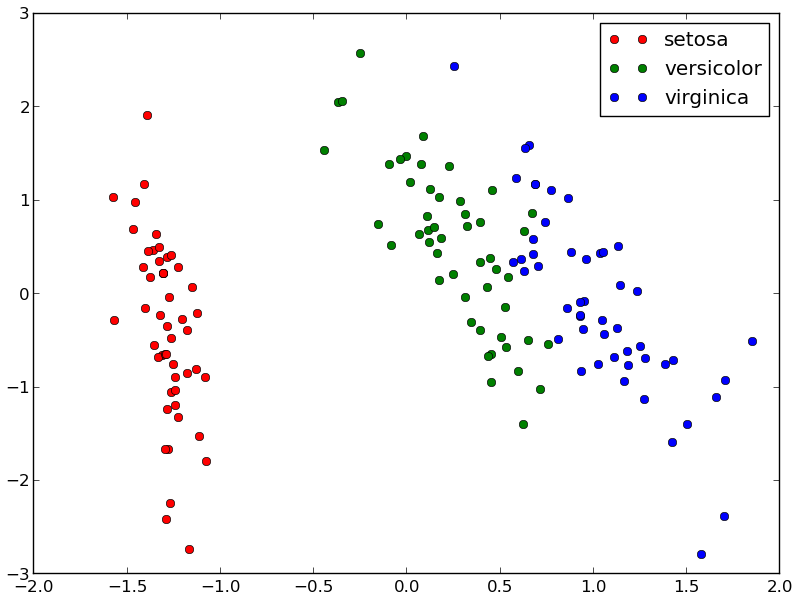
\includegraphics[width=\textwidth]{imgs/plot_iris.png} \\
       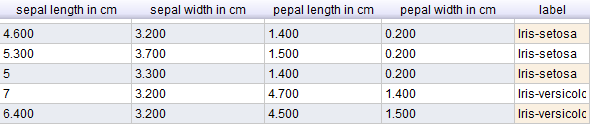
\includegraphics[width=\textwidth]{imgs/iris_dataset.png}
      \end{block}
     \end{column}
     
    \end{columns}

  \end{frame}


\subsection{Relevancia del problema}
  \begin{frame}
    \frametitle{Relevancia del problema}
    
    Todos los datos recolectados por una organización pueden ser útiles para
    mejorar las decisiones futuras de la organización. Para usar los enormes
    volúmenes de datos que se recolectan, es necesario encontrar patrones en
    ellos.
    
  \end{frame}
  

\section{Justificación del uso de IA}
  \begin{frame}
    \frametitle{Justificación del uso de IA}
  \end{frame}

\section{Aplicaciones relevantes}
  \subsection{Aplicación 1}
    \begin{frame}
      \frametitle{Reconocedor de dígitos}
    \end{frame}


%% Bibliografía
\section {Referencias}
\begin{frame}
\frametitle{Referencias}
\footnotesize{
  \begin{thebibliography}{99} % Beamer does not support BibTeX so references must be inserted manually as below
    \bibitem[Herrera, 2015]{h1} Francisco Herrera Triguero
      \newblock Inteligencia Artificial, Inteligencia Computacional y Big Data
      \newblock Capítulo A
      \newblock \emph{Universidad de Jaén (2015)}
  \end{thebibliography}
}
\end{frame}

\end{document} 